\subsection{HPA}
\subsubsection{HPA cpu-utilization}
\begin{figure}[h]
    \begin{minipage}[t]{0.5\textwidth}
        \centering
        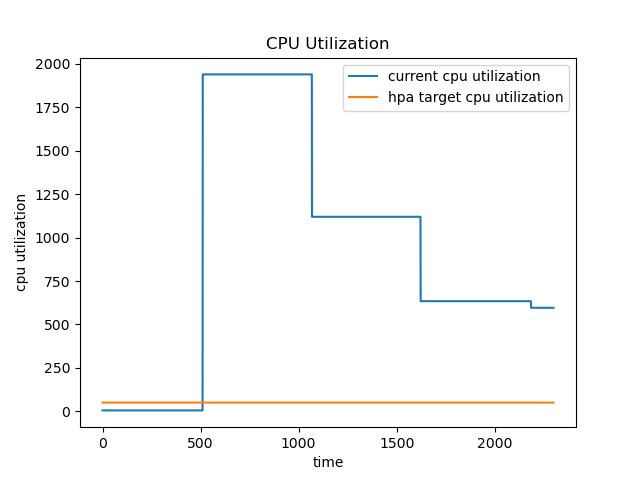
\includegraphics[width=0.9\textwidth]{../sample_results/loop/hpa/cpu-utilization-hpa.png}
        \caption{Loop}
    \end{minipage}
    \hfill
    \begin{minipage}[t]{0.5\textwidth}
        \centering
        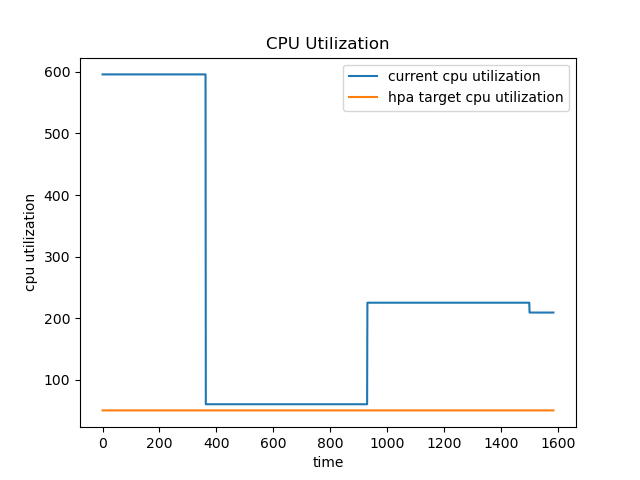
\includegraphics[width=0.9\textwidth]{../sample_results/lorem/hpa/cpu-utilization-hpa.png}
        \caption{Lorem}
    \end{minipage}
\end{figure}
\begin{itemize}
    \item Initial CPU utilization for the HPA configuration is very high due to the limited number of pods available at the start.
    \item As the HPA scales out and increases the number of pods, the workload is distributed across more pods.
    \item Consequently, the CPU utilization per pod decreases over time as more pods are added to handle incoming requests.
    \item This adaptive scaling helps maintain performance while balancing resource usage efficiently.
\end{itemize}

\noindent Below is the replica count graph that illustrates the increase in the number of pods over time, supporting the trend of decreasing CPU utilization per pod:

\begin{figure}[h]
    \begin{minipage}[t]{0.5\textwidth}
        \centering
        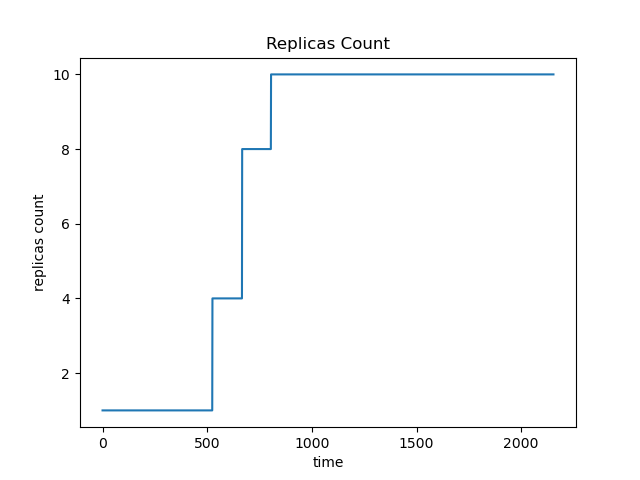
\includegraphics[width=0.9\textwidth]{../sample_results/loop/hpa/replicas-count-hpa.png}
        \caption{Loop}
    \end{minipage}
    \hfill
    \begin{minipage}[t]{0.5\textwidth}
        \centering
        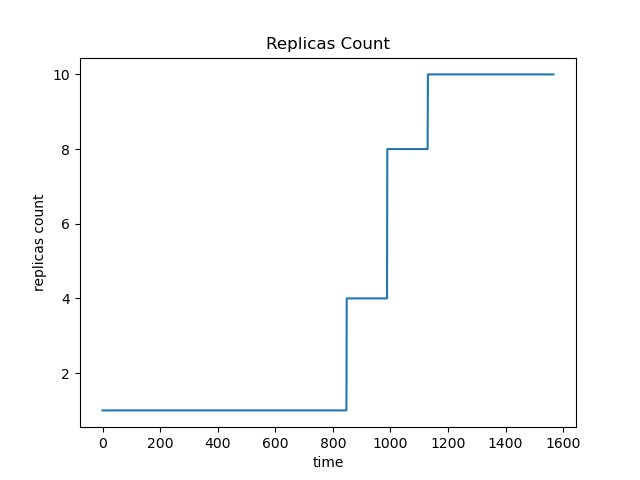
\includegraphics[width=0.9\textwidth]{../sample_results/lorem/hpa/replicas-count-hpa.png}
        \caption{Lorem}
    \end{minipage}
\end{figure}

\subsubsection{HPA Response Time Observations}
\begin{itemize}
    \item Initial response times in the HPA configuration may be higher due to limited pod availability at the start.
    \item As HPA scales out the number of pods in response to increased load, response times start to decrease.
    \item The additional pods allow the service to handle more requests concurrently, resulting in improved response times.
    \item HPA helps maintain consistent response times even as demand fluctuates, by adjusting the number of pods to match the workload.
\end{itemize}

\noindent Below is the response time for HPA.

\begin{figure}[h]
    \begin{minipage}[t]{0.5\textwidth}
        \centering
        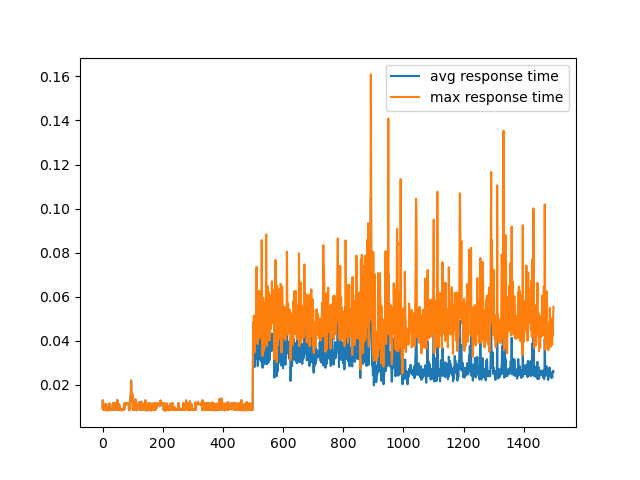
\includegraphics[width=0.9\textwidth]{../sample_results/loop/hpa/response-time-hpa-hpa.png}
        \caption{Loop}
    \end{minipage}
    \hfill
    \begin{minipage}[t]{0.5\textwidth}
        \centering
        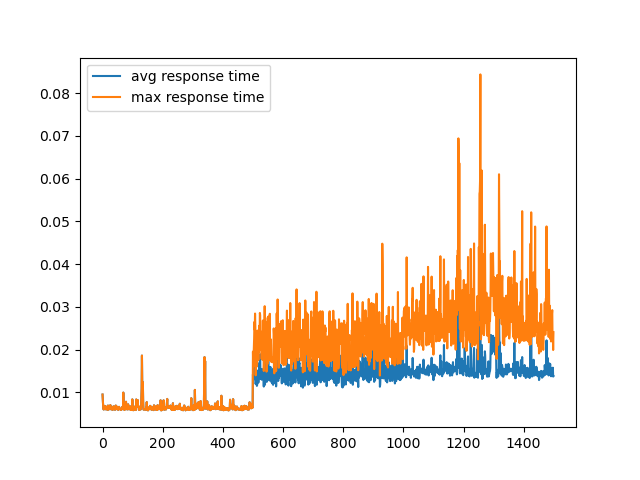
\includegraphics[width=0.9\textwidth]{../sample_results/lorem/hpa/response-time-hpa-hpa.png}
        \caption{Lorem}
    \end{minipage}
\end{figure}

